\section{Method 1: Autoencoders (Erdem Çelikel)}

% --- Slide 1: Dataset Preparation & Architecture ---
\begin{frame}{Dataset Preparation \& Autoencoder Architecture}
    \begin{columns}[c]
        \begin{column}{0.50\textwidth}
            \small
            \begin{itemize}
                \footnotesize
                \item \textbf{Goal \& Motivation:} Swap faces between Person A and Person B while keeping motion. Built custom autoencoder to experience basics before pretrained tools.
                \vspace{0.08cm}
                \item \textbf{Preprocessing:} Recorded short videos, extracted every 5th frame. Haar Cascade detection with \textbf{+25\% margin}. Resized to $128 \times 128$ (0--1 scaled).
                \vspace{0.08cm}
                \item \textbf{Architecture:} 1 shared Encoder (4 conv layers) and 2 Decoders (4 transposed-conv layers each, Sigmoid activation).
                \vspace{0.08cm}
                \item \textbf{Face Swap Scheme:} Pass Person A through Decoder B, and Person B through Decoder A.
            \end{itemize}
        \end{column}

        \begin{column}{0.46\textwidth}
            \centering
            \footnotesize
            \begin{tabular}{lcc}
                \toprule
                \textbf{Subject} & \textbf{Prepared Faces} & \textbf{Resolution} \\
                \midrule
                Person A & 100 & $128 \times 128$ \\
                Person B & 138 & $128 \times 128$ \\
                \midrule
                \textbf{Total} & \textbf{238} & $\mathbf{128 \times 128}$ \\
                \bottomrule
            \end{tabular}

            \vspace{0.15cm}
            \textbf{\footnotesize Input Videos (First Frames)}

            \vspace{0.08cm}
            \begin{columns}[c]
                \begin{column}{0.48\linewidth}
                    \centering
                    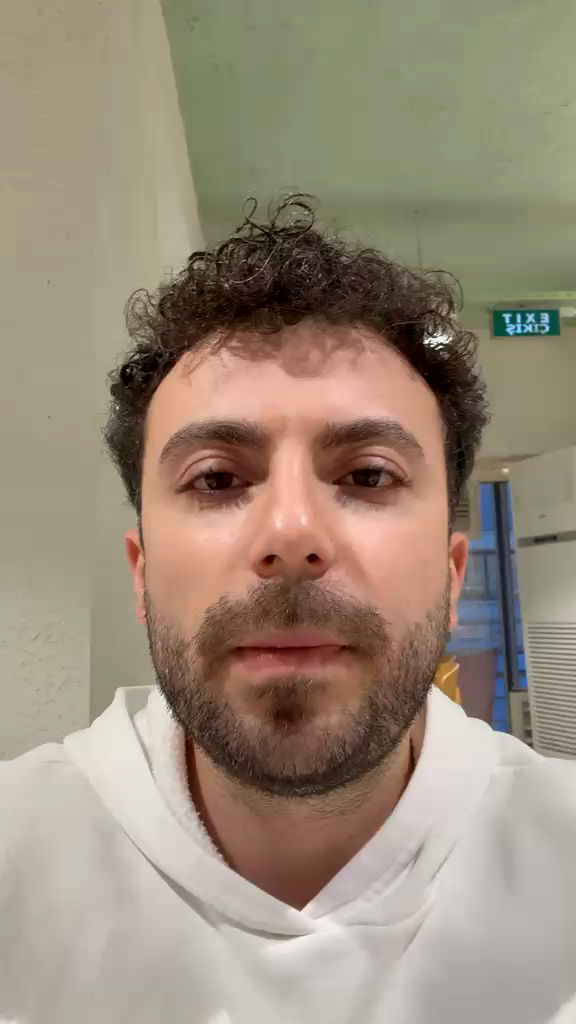
\includegraphics[height=1.8cm, keepaspectratio]{ae_vid_person_a.png} \\
                    \vspace{0.04cm}
                    \scriptsize \textbf{Person A} (100 imgs) \\
                    \href{https://youtu.be/placeholder}{\tiny \underline{\textcolor{primaryNavy}{[person\_A.mp4]}}}
                \end{column}
                \begin{column}{0.48\linewidth}
                    \centering
                    
\includegraphics[height=1.8cm, keepaspectratio]{ae_vid_person_b.png} \\
                    \vspace{0.04cm}
                    \scriptsize \textbf{Person B} (138 imgs) \\
                    \href{https://youtu.be/placeholder}{\tiny \underline{\textcolor{primaryNavy}{[person\_B.mp4]}}}
                \end{column}
            \end{columns}
        \end{column}
    \end{columns}
\end{frame}
